\documentclass[fleqn]{beamer}

\mode<presentation>
{
  \usetheme{default}
%   \useinnertheme[shadow=true]{rounded}

  \useinnertheme{circles}
  
%    \useoutertheme{infolines}
  % or ...
  \setbeamersize{text margin left=1em,text margin right=1em}

%   \setbeamercovered{transparent}
  % or whatever (possibly just delete it)

  \beamertemplatenavigationsymbolsempty
  
% Display frame numbers in footline
  \setbeamertemplate{footline}[frame number]
}

\usepackage{etex}
\usepackage[utf8]{inputenc}
\usepackage[T1]{fontenc}
\usepackage[ngerman]{babel}
\usepackage{amsmath}
% \usepackage{amsthm}
% \usepackage{stmaryrd}
\usepackage{times}
\usepackage{mathpartir}

\usepackage{centernot}

\usepackage{colortbl}
\usepackage{multirow}

\usepackage[purexy]{qsymbols}
\usepackage{graphicx}

\usepackage{listings}
\usepackage{lstautogobble}

\usepackage{ifthen}
\usepackage{pgf}
\usepackage{tikz}
\usetikzlibrary{scopes}
\usetikzlibrary{decorations}
  \usetikzlibrary{decorations.pathmorphing}
\usetikzlibrary{arrows}
\usetikzlibrary{automata}
\usetikzlibrary{positioning}
\usetikzlibrary{chains}
\usetikzlibrary{shapes.geometric}
\usetikzlibrary{shapes.callouts}
\usetikzlibrary{shapes.misc}
\usetikzlibrary{fit}
\usetikzlibrary{calc}
\usepackage{pgfplots}

% \tikzstyle{stack}=[inner sep=0pt,minimum size=2mm]
% \tikzstyle{ssline}=[->,snake=snake,segment amplitude=.2mm,segment length=3mm,line after snake=1mm]
% \tikzstyle{fgnode}=[circle,draw,inner sep=0pt,minimum size=2mm]


\usepackage{packages/isabelle}
\usepackage{packages/isabelletags}
\usepackage{packages/isabellesym}
\usepackage{packages/comment}

% \isabellestyle{it}

\def\isachardoublequote{}%
\def\isachardoublequoteopen{}%
\def\isachardoublequoteclose{}%

\newcommand{\isainnerkeyword}[1]{{\textbf{#1}}}
\newcommand{\isasymexistsA}{\isamath{\exists_{\textsc A}\,}}

\def\isadelimproof{}
\def\endisadelimproof{}
\def\isatagproof{}
\def\endisatagproof{}
\def\isafoldproof{}
\def\isadelimproof{}
\def\endisadelimproof{}

\def\isastylescript{\sl}%


% Not really meant for highlighting isabelle source, but for easily writing latex that looks like
% isabelle
% 
% keyword level 1 - isabelle outer syntax 
% keyword level 2 - isabelle inner syntax programming constructs (if, let, etc)
% keyword level 3 - standard constants (length, mod, etc)
% keyword level 4 - isabelle proof methods

\lstdefinelanguage{isabelle}{
  morekeywords={theorem,theorems,corollary,lemma,lemmas,locale,begin,end,fixes,assumes,shows,
    constrains , definition, where, apply, done,unfolding, primrec, using, by, for, uses,
    schematic_lemma, concrete_definition, prepare_code_thms, export_code, datatype,
    proof, next, qed, show, have, hence, thus, interpretation, fix, context
 } ,
  morekeywords=[2]{rec, return, bind, foreach, if, then, else, and, do, let, in, res, spec, fail, assert, while, case, of},
%  morekeywords=[3]{length,mod,insert},
%   morekeywords=[4]{simp,auto,intro,elim,rprems,refine_mono,refine_rcg},
  sensitive=True,
  morecomment=[s]{(\*}{\*)},
}

\lstset{
    language=isabelle,
    mathescape=true,
    escapeinside={--"}{"},
    basicstyle={\itshape},
    keywordstyle=\rm\bfseries,
    keywordstyle=[2]\rm\tt,
    keywordstyle=[3]\rm,
    keywordstyle=[4]\rm,
    showstringspaces=false,
    keepspaces=true,
    columns=[c]fullflexible}
\lstset{literate=
  {"}{}0
  {'}{{${}^\prime$}}1
  {\%}{{$\lambda$}}1
  {\\\%}{{$\lambda$}}1
  {\\\$}{{$\mathbin{\,\$\,}$}}1
  {->}{{$\rightarrow$}}1
  {<-}{{$\leftarrow$}}1
  {<.}{{$\langle$}}1
  {.>}{{$\rangle$}}1
  {<=}{{$\le$}}1
  {<->}{{$\leftrightarrow$}}1
  {-->}{{$\longrightarrow$}}2
  {<-->}{{$\longleftrightarrow$}}1
  {=>}{{$\Rightarrow$}}1
  {==}{{$\equiv$}}2
  {==>}{{$\implies$}}2
  {<=>}{{$\Leftrightarrow$}}1
  {~=}{{$\ne$}}1
  {!!}{{$\bigwedge$}}1
  {(}{{$($}}1
  {)}{{$)$}}1
  {\{}{{$\{$}}1
  {\}}{{$\}$}}1
  {[}{{$[$}}1
  {]}{{$]$}}1
  {(|}{{$\lrec$}}1
  {|)}{{$\rrec$}}1
  {[|}{{$\lsem$}}1
  {|]}{{$\rsem$}}1
  {\\<lbrakk>}{{$\lsem$}}1
  {\\<rbrakk>}{{$\rsem$}}1
  {|-}{{$\vdash$}}1
  {|->}{{$\mapsto$}}1
  {|_|}{{$\bigsqcup$}}1
  {...}{{$\dots$}}1
  {\\x}{{$\times$}}1
  {_0}{{${}_0$}}1
  {_1}{{${}_1$}}1
  {_2}{{${}_2$}}1
  {_3}{{${}_3$}}1
  {_4}{{${}_4$}}1
  {_5}{{${}_5$}}1
  {_6}{{${}_6$}}1
  {_7}{{${}_7$}}1
  {_8}{{${}_8$}}1
  {_9}{{${}_9$}}1
  {^*}{{$^*$}}1
  {\\<^sup>*}{{$^*$}}1
  {\\<^sub>*}{{$_*$}}1
  {\\<^sub>A}{{$_A$}}1
  {\\<^sub>r}{{$_r$}}1
  {\\<^sub>a}{{$_a$}}1
  {:_i}{{$:_i$}}1
  {\\<A>}{{$\mathcal{A}$}}1
  {\\<O>}{{\sf o}}1
  {\\<Phi>}{{$\Phi$}}1
  {\\<Psi>}{{$\Psi$}}1
  {\\<sigma>}{{$\sigma$}}1
  {\\<in>}{{$\in$}}1
  {\\<le>}{{$\le$}}1
  {\\<noteq>}{{$\ne$}}1
  {\\<lambda>}{{$\lambda$}}1
  {\\<longrightarrow>}{{$\longrightarrow$}}1
  {\\<longleftrightarrow>}{{$\longleftrightarrow$}}1
  {\\<Rightarrow>}{{$\Rightarrow$}}1
  {\\<Longrightarrow>}{{$\Longrightarrow$}}1
  {\\<rightarrow>}{{$\rightarrow$}}1
  {\\<leftarrow>}{{$\leftarrow$}}1
  {\\<mapsto>}{{$\mapsto$}}1
  {\\<equiv>}{{$\equiv$}}1
  {\\<and>}{{$\and$}}1
  {\\<or>}{{$\vee$}}1
  {\\<And>}{{$\bigwedge$}}1
  {\\<Up>}{{$\Uparrow$}}1
  {\\<Down>}{{$\Downarrow$}}1
  {\\<up>}{{$\uparrow$}}1
  {\\<down>}{{$\downarrow$}}1
  {\\<times>}{{$\times$}}1
  {\\<forall>}{{$\forall$}}1
  {\\<exists>}{{$\exists$}}1
  {\\<union>}{{$\cup$}}1
  {\\<Union>}{{$\bigcup$}}1
  {\\<inter>}{{$\cap$}}1
  {\\<subset>}{{$\subset$}}1
  {\\<subseteq>}{{$\subseteq$}}1
  {\\<supset>}{{$\supset$}}1
  {\\<supseteq>}{{$\supseteq$}}1
  {\\<alpha>}{{$\alpha$}}1
  {\\<beta>}{{$\beta$}}1
  {\\<gamma>}{{$\gamma$}}1
  {\\alpha}{{$\alpha$}}1
  {\\beta}{{$\beta$}}1
  {\\gamma}{{$\gamma$}}1
  {\\<Gamma>}{{$\Gamma$}}1
  {\\<langle>}{{$\langle$}}1
  {\\<rangle>}{{$\rangle$}}1
  {\\<not>}{{$\neg$}}1
  {\\<notin>}{{$\notin$}}1
  {\\<guillemotright>}{{$\gg$}}1
  {\\in}{$\in$}1
  {\\and}{$\wedge$}1
  {\\or}{$\vee$}1
  {\\Phi}{{$\Phi$}}1
  {\\Psi}{{$\Psi$}}1
  {\\le}{{$\le$}}1
  {\\Up}{{$\Uparrow$}}1
  {\\Down}{{$\Down$}}1
  {>>}{{$\gg$}}1
  {>>=}{{${\gg}{=}$}}1
  {<*lex*>}{{$\times_{\sf lex}$}}1
}

\newcommand{\isai}{\lstinline[language=isabelle]}

\newcommand\Until{}
% General
\newcommand{\ie}{i.\,e.\ }
\newcommand{\eg}{e.\,g.\ }
\newcommand{\wrt}{wrt.\ }
\newcommand{\cf}{cf.\ }
\newcommand{\etc}{etc.\ }


%Isabelle/HOL
\newcommand{\SOME}{\varepsilon}
\newcommand{\union}{\cup}
\newcommand{\inter}{\cap}
\renewcommand{\and}{\land}

\newcommand{\set}{{\sf set}}

\newcommand{\Sup}{\bigsqcup}
\newcommand{\sle}{\sqsubseteq}

\newcommand{\la}{{\sf \gets}}

\newcommand{\True}{{\sf True}}
\newcommand{\False}{{\sf False}}
\newcommand{\nat}{{\mathbb N}}
\newcommand{\bool}{{\mathbb B}}
\newcommand{\unit}{{\sf unit}}
\newcommand{\last}{{\sf last}}
\newcommand{\butlast}{{\sf butlast}}

\newcommand{\V}{V}

\renewcommand{\implies}{\Longrightarrow}

\newcommand{\isaconst}[1]{\textsl{#1}}
\newcommand{\isakeyw}[1]{\textsf{\bf #1}}
\newcommand{\isalem}[1]{\textsf{#1}}

\newcommand{\locale}{\isakeyw{locale}}

\newcommand{\lrec}{\mathopen{(\!|}}
\newcommand{\rrec}{\mathclose{|\!)}}

\newcommand{\lsem}{\ensuremath{\mathopen{[\![}}}
\newcommand{\rsem}{\ensuremath{\mathclose{]\!]}}}

\newcommand{\up}{\uparrow}

% Refinement Framework
\newcommand{\SUCCEED}{{\sf\bf succeed}}
\newcommand{\FAIL}{{\sf\bf fail}}
\newcommand{\fail}{{\sf\bf fail}}
\newcommand{\RES}{{\sf\bf res}}
\newcommand{\SPEC}{{\sf\bf spec}}
\newcommand{\return}{\RETURN}
\newcommand{\bind}{\BIND}
\newcommand{\RETURN}{{\sf\bf return}}
\newcommand{\BIND}{{\sf\bf bind}}
\newcommand{\assert}{\ASSERT}
\newcommand{\ASSERT}{{\sf\bf assert}}
\renewcommand{\do}{\DO}
\newcommand{\DO}{{\sf\bf do}}
\newcommand{\IN}{{\sf\bf in}}
\newcommand{\IF}{{\sf\bf if}}
\newcommand{\THEN}{{\sf\bf then}}
\newcommand{\ELSE}{{\sf\bf else}}
\newcommand{\LET}{{\sf\bf let}}
\newcommand{\WHILE}{{\sf\bf while}}
\newcommand{\WHILET}{\WHILE_{\sf\bf T}}
\newcommand{\FOREACH}{{\sf\bf foreach}}
\newcommand{\FOREACHC}{\FOREACH_{\sf\bf C}}
\newcommand{\REC}{{\sf\bf rec}}
\newcommand{\RECT}{{\sf\bf rec_T}}

\newcommand{\Up}{{\Uparrow}}
\newcommand{\Down}{{\Downarrow}}

\newcommand{\lfp}{{\sf lfp}}
\newcommand{\gfp}{{\sf gfp}}
\newcommand{\body}{{\sf B}}
\newcommand{\htrip}[3]{{\models\{#1\}~{#2}~\{#3\}}}

\newcommand{\mono}{{\sf mono}}
\newcommand{\wf}{{\sf wf}}

%LTL
\newcommand{\Prop}{\mathsf{Prop}}
\newcommand{\Next}{\mathord{\mathsf{X}}}
\newcommand{\Finally}{\mathord{\mathsf{F}}}
\newcommand{\Globally}{\mathord{\mathsf{G}}}
\renewcommand{\Until}{\mathbin{\mathsf{U}}}
\newcommand{\Release}{\mathbin{\mathsf{V}}}

%Automata
\newcommand{\GBA}{\mathord{\mathsf{GBA}}}
\newcommand{\LGBA}{\mathord{\mathsf{LGBA}}}

\newcommand{\QGBA}{{{Q\_GBA}}}
\newcommand{\DGBA}{{{\Delta\_GBA}}}
\newcommand{\IGBA}{{{I\_GBA}}}
\newcommand{\FGBA}{{{F\_GBA}}}
\newcommand{\LLGBA}{{{L}}}

\newcommand{\BAtrans}{\mathsf{trans}}
\newcommand{\BAinitial}{\mathsf{initial}}
\newcommand{\BAaccept}{\mathsf{accept}}

%Misc
\newcommand{\equivalent}{\leftrightarrow}

\newcommand{\expand}{\mathbin{\mathsf{expand}}}
\newcommand{\expandbody}{\mathbin{\mathsf{expand\_body}}}
\def\by#1{\mathop{{\hbox{\setbox0=\hbox{$\scriptstyle{#1\quad}$}{$\buildrel{\>#1\>}\over{\hbox to \wd0{\rightarrowfill}}$}}}}}

%personalized comments
\newcommand{\as}[1]{\textcolor{blue}{\sf AS: #1}}
\newcommand{\AS}[1]{\marginpar{\footnotesize\textcolor{blue}{\sf AS: #1}}}
\newcommand{\RN}[1]{\marginpar{\footnotesize\textcolor{green}{\sf RN: #1}}}
\newcommand{\JE}[1]{\marginpar{\footnotesize\textcolor{green}{\sf JE: #1}}}
\newcommand{\PL}[1]{\marginpar{\footnotesize\textcolor{red}{\sf PL: #1}}}
\newcommand{\jgs}[1]{\textcolor{magenta}{\sf jgs: #1}}
\newcommand{\JGS}[1]{\marginpar{\footnotesize\textcolor{magenta}{\sf JGS: #1}}}



\newcommand{\eqdef}{\mathrel{{=}_{def}}}
\newcommand{\iffdef}{\mathrel{{\mathord{\iff}\!\!}_{def}}}


\makeatletter
\newcommand*{\overlaynumber}{\number\beamer@slideinframe}
\makeatother

\AtBeginSection[] % Do nothing for \section*
{
  \begin{frame}<beamer>
    \frametitle{Outline}
    \tableofcontents[currentsection]
  \end{frame}
}


\title{Formalizing the Edmonds-Karp Algorithm}

% \subtitle
% {Subtitle} % (optional)

\author[Peter Lammich]{Peter Lammich and S.~Reza Sefidgar}
% - Use the \inst{?} command only if the authors have different
%   affiliation.

\institute[TUM] % (optional, but mostly needed)
{ TU M\"unchen %, Institut f\"ur Informatik, Chair for Logic and Verification
}
% - Use the \inst command only if there are several affiliations.
% - Keep it simple, no one is interested in your street address.

\date {August 2016}
% {2008-12-01}


% If you have a file called "university-logo-filename.xxx", where xxx
% is a graphic format that can be processed by latex or pdflatex,
% resp., then you can add a logo as follows:

% \pgfdeclareimage[height=0.5cm]{university-logo}{university-logo-filename}
% \logo{\pgfuseimage{university-logo}}


% Delete this, if you do not want the table of contents to pop up at
% the beginning of each subsection:


% If you wish to uncover everything in a step-wise fashion, uncomment
% the following command: 

%\beamerdefaultoverlayspecification{<+->}

%\mathchardef\-="2D
%\renewcommand\-{\text{-}}

\newcommand{\mc}{\color{blue}}
\newcommand{\term}[1]{{\mc#1}}

\let\olddisplaystyle\displaystyle
\newcommand{\mydisplaystyle}{\olddisplaystyle\mc}
\let\displaystyle\mydisplaystyle

\newcommand{\smc}{\everymath{\mc}}
\smc

% \newcommand<>{\btikzset}[2]{\alt#3{\tikzset{#1}}{\tikzset{#2}}}

\tikzset{onslide/.code args={<#1>#2}{%
  \only<#1>{\pgfkeysalso{#2}} % \pgfkeysalso doesn't change the path
}}

\tikzset{>=latex}


\lstset{autogobble}

\newcommand{\natN}{{\text{nat}_{\mathord{<}N}}}

\newcommand{\edge}[1]{\stackrel{#1}{\longrightarrow}}

\begin{document}
% % General
\newcommand{\ie}{i.\,e.\ }
\newcommand{\eg}{e.\,g.\ }
\newcommand{\wrt}{wrt.\ }
\newcommand{\cf}{cf.\ }
\newcommand{\etc}{etc.\ }


%Isabelle/HOL
\newcommand{\SOME}{\varepsilon}
\newcommand{\union}{\cup}
\newcommand{\inter}{\cap}
\renewcommand{\and}{\land}

\newcommand{\set}{{\sf set}}

\newcommand{\Sup}{\bigsqcup}
\newcommand{\sle}{\sqsubseteq}

\newcommand{\la}{{\sf \gets}}

\newcommand{\True}{{\sf True}}
\newcommand{\False}{{\sf False}}
\newcommand{\nat}{{\mathbb N}}
\newcommand{\bool}{{\mathbb B}}
\newcommand{\unit}{{\sf unit}}
\newcommand{\last}{{\sf last}}
\newcommand{\butlast}{{\sf butlast}}

\newcommand{\V}{V}

\renewcommand{\implies}{\Longrightarrow}

\newcommand{\isaconst}[1]{\textsl{#1}}
\newcommand{\isakeyw}[1]{\textsf{\bf #1}}
\newcommand{\isalem}[1]{\textsf{#1}}

\newcommand{\locale}{\isakeyw{locale}}

\newcommand{\lrec}{\mathopen{(\!|}}
\newcommand{\rrec}{\mathclose{|\!)}}

\newcommand{\lsem}{\ensuremath{\mathopen{[\![}}}
\newcommand{\rsem}{\ensuremath{\mathclose{]\!]}}}

\newcommand{\up}{\uparrow}

% Refinement Framework
\newcommand{\SUCCEED}{{\sf\bf succeed}}
\newcommand{\FAIL}{{\sf\bf fail}}
\newcommand{\fail}{{\sf\bf fail}}
\newcommand{\RES}{{\sf\bf res}}
\newcommand{\SPEC}{{\sf\bf spec}}
\newcommand{\return}{\RETURN}
\newcommand{\bind}{\BIND}
\newcommand{\RETURN}{{\sf\bf return}}
\newcommand{\BIND}{{\sf\bf bind}}
\newcommand{\assert}{\ASSERT}
\newcommand{\ASSERT}{{\sf\bf assert}}
\renewcommand{\do}{\DO}
\newcommand{\DO}{{\sf\bf do}}
\newcommand{\IN}{{\sf\bf in}}
\newcommand{\IF}{{\sf\bf if}}
\newcommand{\THEN}{{\sf\bf then}}
\newcommand{\ELSE}{{\sf\bf else}}
\newcommand{\LET}{{\sf\bf let}}
\newcommand{\WHILE}{{\sf\bf while}}
\newcommand{\WHILET}{\WHILE_{\sf\bf T}}
\newcommand{\FOREACH}{{\sf\bf foreach}}
\newcommand{\FOREACHC}{\FOREACH_{\sf\bf C}}
\newcommand{\REC}{{\sf\bf rec}}
\newcommand{\RECT}{{\sf\bf rec_T}}

\newcommand{\Up}{{\Uparrow}}
\newcommand{\Down}{{\Downarrow}}

\newcommand{\lfp}{{\sf lfp}}
\newcommand{\gfp}{{\sf gfp}}
\newcommand{\body}{{\sf B}}
\newcommand{\htrip}[3]{{\models\{#1\}~{#2}~\{#3\}}}

\newcommand{\mono}{{\sf mono}}
\newcommand{\wf}{{\sf wf}}

%LTL
\newcommand{\Prop}{\mathsf{Prop}}
\newcommand{\Next}{\mathord{\mathsf{X}}}
\newcommand{\Finally}{\mathord{\mathsf{F}}}
\newcommand{\Globally}{\mathord{\mathsf{G}}}
\renewcommand{\Until}{\mathbin{\mathsf{U}}}
\newcommand{\Release}{\mathbin{\mathsf{V}}}

%Automata
\newcommand{\GBA}{\mathord{\mathsf{GBA}}}
\newcommand{\LGBA}{\mathord{\mathsf{LGBA}}}

\newcommand{\QGBA}{{{Q\_GBA}}}
\newcommand{\DGBA}{{{\Delta\_GBA}}}
\newcommand{\IGBA}{{{I\_GBA}}}
\newcommand{\FGBA}{{{F\_GBA}}}
\newcommand{\LLGBA}{{{L}}}

\newcommand{\BAtrans}{\mathsf{trans}}
\newcommand{\BAinitial}{\mathsf{initial}}
\newcommand{\BAaccept}{\mathsf{accept}}

%Misc
\newcommand{\equivalent}{\leftrightarrow}

\newcommand{\expand}{\mathbin{\mathsf{expand}}}
\newcommand{\expandbody}{\mathbin{\mathsf{expand\_body}}}
\def\by#1{\mathop{{\hbox{\setbox0=\hbox{$\scriptstyle{#1\quad}$}{$\buildrel{\>#1\>}\over{\hbox to \wd0{\rightarrowfill}}$}}}}}

%personalized comments
\newcommand{\as}[1]{\textcolor{blue}{\sf AS: #1}}
\newcommand{\AS}[1]{\marginpar{\footnotesize\textcolor{blue}{\sf AS: #1}}}
\newcommand{\RN}[1]{\marginpar{\footnotesize\textcolor{green}{\sf RN: #1}}}
\newcommand{\JE}[1]{\marginpar{\footnotesize\textcolor{green}{\sf JE: #1}}}
\newcommand{\PL}[1]{\marginpar{\footnotesize\textcolor{red}{\sf PL: #1}}}
\newcommand{\jgs}[1]{\textcolor{magenta}{\sf jgs: #1}}
\newcommand{\JGS}[1]{\marginpar{\footnotesize\textcolor{magenta}{\sf JGS: #1}}}



\begin{frame}
  \titlepage
\end{frame}

# Maximum Flow Problem
  * Network: Digraph with edge capacities and source/sink nodes
  * Flow: From source to sink, not exceeding capacities
    * Kirchhoff's law: Inflow = Outflow for all nodes but source/sink
    * No inflow to source, no outflow from sink
    * Value: Flow transported from source to sink (=Outflow of source)
  * Problem: Given a network, find a flow with maximal value

# Ford-Fulkerson Method
  * Consider network with flow
    * No antiparallel edges: $u\edge{} v \implies v\centernot{\edge{}} u$
  * Residual graph
    * For network edge $u\edge{c,f} v$, residual graph has
      \[ u\edge{c-f} v \text{ and } v\edge{f} u \]
    * Intuition: Flow that can be moved between nodes
      * By either increasing or decreasing flow on network edge
  * Ford-Fulkerson
    * Flow is maximal iff no path from source to sink in residual graph
    * Corollary of min-cut max-flow theorem

#! Ford-Fulkerson Method
  {}
  {\small{Flow is maximal iff no path from source to sink in residual graph.}}
  \vfill

  * Greedy Algorithm
    \begin{lstlisting}
      Set flow to zero
      while exists augmenting path
        augment flow along path
    \end{lstlisting}%
  * Partial correctness: obvious
  * Termination: Only for integer/rational capacities
  * Edmonds/Karp: Choose shortest augmenting path
    * $O(VE)$ iterations for real-valued capacities
    * Using BFS to find path: $O(VE^2)$ algorithm

# Our Contributions 
  {Verified in Isabelle/HOL}

  * Min-Cut Max-Flow theorem
    * Human-Readable Isar proof
    * Closely following Cormen et al.
  * Ford-Fulkerson and Edmonds Karp algorithms
    * Human-readable presentation of algorithms
    * Proved Correctness and Complexity
  * Efficient Implementation
    * Using stepwise refinement down to Imperative/HOL
    * Isabelle's code generator exports to SML
    * Benchmark: Comparable to Java (from Sedgewick et al.)

\newcommand{\augment}{{\mathbin\uparrow}}%

\newcommand{\isasnipb}[1]{{\setbeamercolor{math text}{fg=black}#1}}
\newcommand{\isasnip}[1]{{\footnotesize\isasnipb{#1}}}
\newcommand{\isasnipsmall}[1]{{\scriptsize\isasnipb{#1}}}



\def\isarproofsnippet{
\ \ \isacommand{have}\isamarkupfalse%
\ {\isachardoublequoteopen}{\isacharparenleft}f{\isasymup}f{\isacharprime}{\isacharparenright}{\isacharparenleft}u{\isacharcomma}v{\isacharparenright}\ {\isacharequal}\ f{\isacharparenleft}u{\isacharcomma}v{\isacharparenright}\ {\isacharplus}\ f{\isacharprime}{\isacharparenleft}u{\isacharcomma}v{\isacharparenright}\ {\isacharminus}\ f{\isacharprime}{\isacharparenleft}v{\isacharcomma}u{\isacharparenright}{\isachardoublequoteclose}\ \isanewline
\ \ \ \ \isacommand{by}\isamarkupfalse%
\ {\isacharparenleft}auto\ simp{\isacharcolon}\ augment{\isacharunderscore}def{\isacharparenright}\isanewline
\ \ \isacommand{also}\isamarkupfalse%
\ \isacommand{have}\isamarkupfalse%
\ {\isachardoublequoteopen}{\isasymdots}\ {\isasymle}\ f{\isacharparenleft}u{\isacharcomma}v{\isacharparenright}\ {\isacharplus}\ f{\isacharprime}{\isacharparenleft}u{\isacharcomma}v{\isacharparenright}{\isachardoublequoteclose}\ \isacommand{using}\isamarkupfalse%
\ f{\isacharprime}{\isachardot}capacity{\isacharunderscore}const\ \isacommand{by}\isamarkupfalse%
\ auto\isanewline
\ \ \isacommand{also}\isamarkupfalse%
\ \isacommand{have}\isamarkupfalse%
\ {\isachardoublequoteopen}{\isasymdots}\ {\isasymle}\ f{\isacharparenleft}u{\isacharcomma}v{\isacharparenright}\ {\isacharplus}\ cf{\isacharparenleft}u{\isacharcomma}v{\isacharparenright}{\isachardoublequoteclose}\ \isacommand{using}\isamarkupfalse%
\ f{\isacharprime}{\isachardot}capacity{\isacharunderscore}const\ \isacommand{by}\isamarkupfalse%
\ auto\isanewline
\ \ \isacommand{also}\isamarkupfalse%
\ \isacommand{have}\isamarkupfalse%
\ {\isachardoublequoteopen}{\isasymdots}\ {\isacharequal}\ f{\isacharparenleft}u{\isacharcomma}v{\isacharparenright}\ {\isacharplus}\ c{\isacharparenleft}u{\isacharcomma}v{\isacharparenright}\ {\isacharminus}\ f{\isacharparenleft}u{\isacharcomma}v{\isacharparenright}{\isachardoublequoteclose}\ \isanewline
\ \ \ \ \isacommand{by}\isamarkupfalse%
\ {\isacharparenleft}auto\ simp{\isacharcolon}\ residualGraph{\isacharunderscore}def{\isacharparenright}\isanewline
\ \ \isacommand{also}\isamarkupfalse%
\ \isacommand{have}\isamarkupfalse%
\ {\isachardoublequoteopen}{\isasymdots}\ {\isacharequal}\ c{\isacharparenleft}u{\isacharcomma}v{\isacharparenright}{\isachardoublequoteclose}\ \isacommand{by}\isamarkupfalse%
\ auto\isanewline
\ \ \isacommand{finally}\isamarkupfalse%
\ \isacommand{show}\isamarkupfalse%
\ {\isachardoublequoteopen}{\isacharparenleft}f{\isasymup}f{\isacharprime}{\isacharparenright}{\isacharparenleft}u{\isacharcomma}\ v{\isacharparenright}\ {\isasymle}\ c{\isacharparenleft}u{\isacharcomma}\ v{\isacharparenright}{\isachardoublequoteclose}\ \isacommand{{\isachardot}}\isamarkupfalse%
}

# Human-Readable Proofs
  *<1-> Tried to use Isar in readable way
  
    \begin{uncoverenv}<2->
    {\footnotesize Proof fragment from Cormen at al.:
    \begin{align*}
    (f \uparrow f') (u, v) &= f(u, v) + f'(u, v) - f'(v, u)  && \text{(definition of $\augment$)} \\
    & \leq f(u, v) + f'(u, v) && \text{(because flows are nonnegative)} \\
    & \leq f(u, v) + c_f(u, v) &&  \text{(capacity constraint)} \\
    & = f(u, v) + c(u, v) - f(u, v) && \text{(definition of $c_f$)} \\
    & = c (u, v).
    \end{align*}
    }
    \end{uncoverenv}

    \begin{uncoverenv}<3->
    \isasnip{
      Our Isar version:\\[1em]
      \isarproofsnippet
    }
    \end{uncoverenv}

{
\def\isarsnippetstatement{
\isamarkuptrue%
\isacommand{lemma}\isamarkupfalse%
\ augment{\isacharunderscore}flow{\isacharunderscore}value{\isacharcolon}\ {\isachardoublequoteopen}Flow{\isachardot}val\ c\ s\ {\isacharparenleft}f{\isasymup}f{\isacharprime}{\isacharparenright}\ {\isacharequal}\ val\ {\isacharplus}\ Flow{\isachardot}val\ cf\ s\ f{\isacharprime}{\isachardoublequoteclose}\isanewline
%
\isadelimproof
%
\endisadelimproof
%
\isatagproof
\isacommand{proof}\isamarkupfalse%
\ {\isacharminus}\isanewline
\ \ \isacommand{interpret}\isamarkupfalse%
\ f{\isacharprime}{\isacharprime}{\isacharcolon}\ Flow\ c\ s\ t\ {\isachardoublequoteopen}f{\isasymup}f{\isacharprime}{\isachardoublequoteclose}\ \isacommand{using}\isamarkupfalse%
\ augment{\isacharunderscore}flow{\isacharunderscore}presv{\isacharbrackleft}OF\ assms{\isacharbrackright}\ \isacommand{{\isachardot}}\isamarkupfalse%
}    

\def\isarsnippetsimpset{
\isamarkuptrue%
\ \ \isacommand{note}\isamarkupfalse%
\ setsum{\isacharunderscore}simp{\isacharunderscore}setup{\isacharbrackleft}simp{\isacharbrackright}\ {\isacharequal}\ \isanewline
\ \ \ \ sum{\isacharunderscore}outgoing{\isacharunderscore}alt{\isacharbrackleft}OF\ capacity{\isacharunderscore}const{\isacharbrackright}\ s{\isacharunderscore}node\isanewline
\ \ \ \ sum{\isacharunderscore}incoming{\isacharunderscore}alt{\isacharbrackleft}OF\ capacity{\isacharunderscore}const{\isacharbrackright}\isanewline
\ \ \ \ cf{\isachardot}sum{\isacharunderscore}outgoing{\isacharunderscore}alt{\isacharbrackleft}OF\ f{\isacharprime}{\isachardot}capacity{\isacharunderscore}const{\isacharbrackright}\isanewline
\ \ \ \ cf{\isachardot}sum{\isacharunderscore}incoming{\isacharunderscore}alt{\isacharbrackleft}OF\ f{\isacharprime}{\isachardot}capacity{\isacharunderscore}const{\isacharbrackright}\isanewline
\ \ \ \ sum{\isacharunderscore}outgoing{\isacharunderscore}alt{\isacharbrackleft}OF\ f{\isacharprime}{\isacharprime}{\isachardot}capacity{\isacharunderscore}const{\isacharbrackright}\isanewline
\ \ \ \ sum{\isacharunderscore}incoming{\isacharunderscore}alt{\isacharbrackleft}OF\ f{\isacharprime}{\isacharprime}{\isachardot}capacity{\isacharunderscore}const{\isacharbrackright}\isanewline
\ \ \ \ setsum{\isacharunderscore}subtractf\ setsum{\isachardot}distrib%
}
\def\isarsnippetaux{\isamarkuptrue%
\ \ \isacommand{have}\isamarkupfalse%
\ aux{\isadigit{1}}{\isacharcolon}\ {\isachardoublequoteopen}f{\isacharprime}{\isacharparenleft}u{\isacharcomma}v{\isacharparenright}\ {\isacharequal}\ {\isadigit{0}}{\isachardoublequoteclose}\ \isakeyword{if}\ {\isachardoublequoteopen}{\isacharparenleft}u{\isacharcomma}v{\isacharparenright}{\isasymnotin}E{\isachardoublequoteclose}\ {\isachardoublequoteopen}{\isacharparenleft}v{\isacharcomma}u{\isacharparenright}{\isasymnotin}E{\isachardoublequoteclose}\ \isakeyword{for}\ u\ v\isanewline
\ \ \isacommand{proof}\isamarkupfalse%
\ {\isacharminus}\isanewline
\ \ \ \ \isacommand{from}\isamarkupfalse%
\ that\ cfE{\isacharunderscore}ss{\isacharunderscore}invE\ \isacommand{have}\isamarkupfalse%
\ {\isachardoublequoteopen}{\isacharparenleft}u{\isacharcomma}v{\isacharparenright}{\isasymnotin}cf{\isachardot}E{\isachardoublequoteclose}\ \isacommand{by}\isamarkupfalse%
\ auto\isanewline
\ \ \ \ \isacommand{thus}\isamarkupfalse%
\ {\isachardoublequoteopen}f{\isacharprime}{\isacharparenleft}u{\isacharcomma}v{\isacharparenright}\ {\isacharequal}\ {\isadigit{0}}{\isachardoublequoteclose}\ \isacommand{by}\isamarkupfalse%
\ auto\isanewline
\ \ \isacommand{qed}\isamarkupfalse%
}
\def\isarsnippetredprf{
\isamarkuptrue%
\ \ \isacommand{have}\isamarkupfalse%
\ {\isachardoublequoteopen}f{\isacharprime}{\isacharprime}{\isachardot}val\ {\isacharequal}\ {\isacharparenleft}{\isasymSum}u{\isasymin}V{\isachardot}\ augment\ f{\isacharprime}\ {\isacharparenleft}s{\isacharcomma}\ u{\isacharparenright}\ {\isacharminus}\ augment\ f{\isacharprime}\ {\isacharparenleft}u{\isacharcomma}\ s{\isacharparenright}{\isacharparenright}{\isachardoublequoteclose}\ \isanewline
\ \ \ \ \isacommand{unfolding}\isamarkupfalse%
\ f{\isacharprime}{\isacharprime}{\isachardot}val{\isacharunderscore}def\ \isacommand{by}\isamarkupfalse%
\ simp\isanewline
\ \ \isacommand{also}\isamarkupfalse%
\ \isacommand{have}\isamarkupfalse%
\ {\isachardoublequoteopen}{\isasymdots}\ {\isacharequal}\ {\isacharparenleft}{\isasymSum}u{\isasymin}V{\isachardot}\ f\ {\isacharparenleft}s{\isacharcomma}\ u{\isacharparenright}\ {\isacharminus}\ f\ {\isacharparenleft}u{\isacharcomma}\ s{\isacharparenright}\ {\isacharplus}\ {\isacharparenleft}f{\isacharprime}\ {\isacharparenleft}s{\isacharcomma}\ u{\isacharparenright}\ {\isacharminus}\ f{\isacharprime}\ {\isacharparenleft}u{\isacharcomma}\ s{\isacharparenright}{\isacharparenright}{\isacharparenright}{\isachardoublequoteclose}\isanewline
\ \ \ \ %
\isamarkupcmt{Note that this is the crucial step of the proof, which Cormen et al. leave as an exercise.%
}
\isanewline
\ \ \ \ \isacommand{by}\isamarkupfalse%
\ {\isacharparenleft}rule\ setsum{\isachardot}cong{\isacharparenright}\ {\isacharparenleft}auto\ simp{\isacharcolon}\ augment{\isacharunderscore}def\ no{\isacharunderscore}parallel{\isacharunderscore}edge\ aux{\isadigit{1}}{\isacharparenright}\isanewline
\ \ \isacommand{also}\isamarkupfalse%
\ \isacommand{have}\isamarkupfalse%
\ {\isachardoublequoteopen}{\isasymdots}\ {\isacharequal}\ val\ {\isacharplus}\ Flow{\isachardot}val\ cf\ s\ f{\isacharprime}{\isachardoublequoteclose}\ \ \isanewline
\ \ \ \ \isacommand{unfolding}\isamarkupfalse%
\ val{\isacharunderscore}def\ f{\isacharprime}{\isachardot}val{\isacharunderscore}def\ \isacommand{by}\isamarkupfalse%
\ simp\isanewline
\ \ \isacommand{finally}\isamarkupfalse%
\ \isacommand{show}\isamarkupfalse%
\ {\isachardoublequoteopen}f{\isacharprime}{\isacharprime}{\isachardot}val\ {\isacharequal}\ val\ {\isacharplus}\ f{\isacharprime}{\isachardot}val{\isachardoublequoteclose}\ \isacommand{{\isachardot}}\isamarkupfalse%
\ \ \isanewline
\isacommand{qed}\isamarkupfalse%
}
    
#[t] And Automatic Proofs
  {}
  
  *<1-> Cormen et al. also give more complicated proofs
  *<2-> We sometimes chose to use more automatic proofs
    *<3-> Using some simplifier setup
    *<4-> And auxiliary statements
    *<5-> We reduce the displayed proof's complexity
  
  \vfill
  \begin{onlyenv}<1>
  First part of proof that $|f\up f'| = |f|+|f'|$:\\
  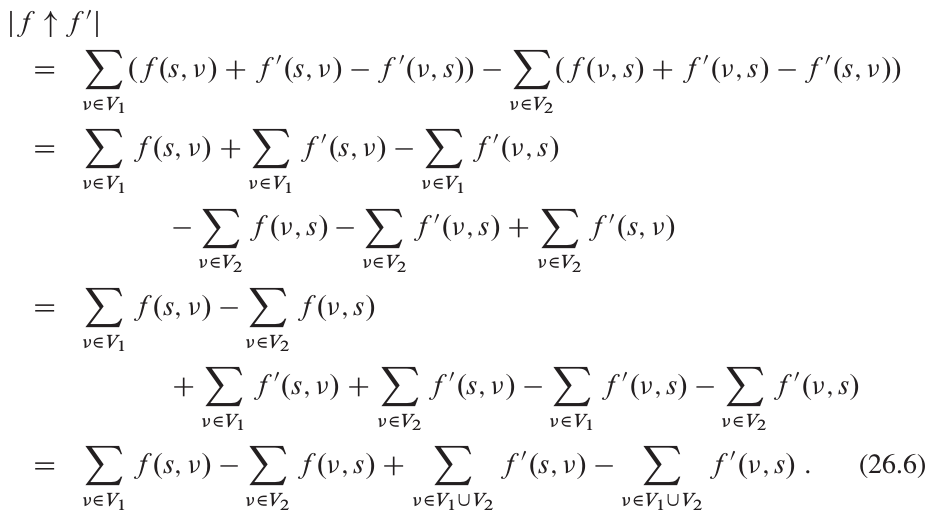
\includegraphics[width=.7\textwidth]{cormen26_6.png}
  \end{onlyenv}
  \begin{onlyenv}<2>
    \isasnip\isarsnippetstatement
  \end{onlyenv}
  \begin{onlyenv}<3>
    \isasnip\isarsnippetsimpset
  \end{onlyenv}
  \begin{onlyenv}<4>
    \isasnip\isarsnippetaux
  \end{onlyenv}
  \begin{onlyenv}<5>
    \isasnip\isarsnippetredprf
  \end{onlyenv}
  
}  

{
\def\snippetfofuthm{
\isamarkuptrue%
\isacommand{context}\isamarkupfalse%
\ NFlow\ \isakeyword{begin}%
\isanewline...\isanewline
\isamarkuptrue%
\isacommand{theorem}\isamarkupfalse%
\ ford{\isacharunderscore}fulkerson{\isacharcolon}\ \isakeyword{shows}\isanewline
\ \ {\isachardoublequoteopen}isMaxFlow\ f\ {\isasymlongleftrightarrow}\ {\isasymnot}\ Ex\ isAugmentingPath{\isachardoublequoteclose}\ 
}
# Main Result
 * Finally, we arrive at\\[2em]
    \isasnip\snippetfofuthm

}


{
\def\snippetfofu{
\isacommand{definition}\isamarkupfalse%
\ {\isachardoublequoteopen}ford{\isacharunderscore}fulkerson{\isacharunderscore}method\ {\isasymequiv}\ \isainnerkeyword{do}\ {\isacharbraceleft}\isanewline
\ \ \isainnerkeyword{let}\ f\ {\isacharequal}\ {\isacharparenleft}{\isasymlambda}{\isacharparenleft}u{\isacharcomma}v{\isacharparenright}{\isachardot}\ {\isadigit{0}}{\isacharparenright}{\isacharsemicolon}\isanewline
\isanewline
\ \ {\isacharparenleft}f{\isacharcomma}brk{\isacharparenright}\ {\isasymleftarrow}\ \isainnerkeyword{while}\ {\isacharparenleft}{\isasymlambda}{\isacharparenleft}f{\isacharcomma}brk{\isacharparenright}{\isachardot}\ {\isasymnot}brk{\isacharparenright}\ \isanewline
\ \ \ \ {\isacharparenleft}{\isasymlambda}{\isacharparenleft}f{\isacharcomma}brk{\isacharparenright}{\isachardot}\ \isainnerkeyword{do}\ {\isacharbraceleft}\isanewline
\ \ \ \ \ \ p\ {\isasymleftarrow}\ \isainnerkeyword{selectp}\ p{\isachardot}\ is{\isacharunderscore}augmenting{\isacharunderscore}path\ f\ p{\isacharsemicolon}\isanewline
\ \ \ \ \ \ \isainnerkeyword{case}\ p\ of\ \isanewline
\ \ \ \ \ \ \ \ None\ {\isasymRightarrow}\ \isainnerkeyword{return}\ {\isacharparenleft}f{\isacharcomma}True{\isacharparenright}\isanewline
\ \ \ \ \ \ {\isacharbar}\ Some\ p\ {\isasymRightarrow}\ \isainnerkeyword{return}\ {\isacharparenleft}augment\ c\ f\ p{\isacharcomma}\ False{\isacharparenright}\isanewline
\ \ \ \ {\isacharbraceright}{\isacharparenright}\isanewline
\ \ \ \ {\isacharparenleft}f{\isacharcomma}False{\isacharparenright}{\isacharsemicolon}\isanewline
\ \ \isainnerkeyword{return}\ f\ \isanewline
{\isacharbraceright}{\isachardoublequoteclose}%
}
%%BEGIN-FILTER: sed -rf massage_snippets.sed
\def\snippetproof{
\isamarkuptrue%
\isacommand{theorem}\isamarkupfalse%
\ fofu{\isacharunderscore}partial{\isacharunderscore}correct{\isacharcolon}\ {\isachardoublequoteopen}fofu\ {\isasymle}\ {\isacharparenleft}{spec}\ f{\isachardot}\ isMaxFlow\ f{\isacharparenright}{\isachardoublequoteclose}\isanewline
%
\isadelimproof
\ \ %
\endisadelimproof
%
\isanewline
\isatagproof
\isacommand{unfolding}\isamarkupfalse%
\ fofu{\isacharunderscore}def\ find{\isacharunderscore}augmenting{\isacharunderscore}spec{\isacharunderscore}def\isanewline
\ \ \isacommand{apply}\isamarkupfalse%
\ {\isacharparenleft}refine{\isacharunderscore}vcg{\isacharparenright}\isanewline
\ \ \isacommand{apply}\isamarkupfalse%
\ {\isacharparenleft}vc{\isacharunderscore}solve\ simp{\isacharcolon}\ \isanewline
\ \ \ \ zero{\isacharunderscore}flow\ \isanewline
\ \ \ \ NFlow{\isachardot}augment{\isacharunderscore}pres{\isacharunderscore}nflow\ \isanewline
\ \ \ \ NFlow{\isachardot}augmenting{\isacharunderscore}path{\isacharunderscore}not{\isacharunderscore}empty\isanewline
\ \ \ \ NFlow{\isachardot}noAugPath{\isacharunderscore}iff{\isacharunderscore}maxFlow{\isacharbrackleft}symmetric{\isacharbrackright}{\isacharparenright}\isanewline
\ \ \isacommand{done}\isamarkupfalse%
%
\endisatagproof%
}
\def\snippetfofuassn{
\isamarkuptrue%
\isacommand{definition}\isamarkupfalse%
\ {\isachardoublequoteopen}fofu\ {\isasymequiv}\ do\ {\isacharbraceleft}\isanewline
\ \ let\ f\ {\isacharequal}\ {\isacharparenleft}{\isasymlambda}{\isacharunderscore}{\isachardot}\ {\isadigit{0}}{\isacharparenright}{\isacharsemicolon}\isanewline
\isanewline
\ \ {\isacharparenleft}f{\isacharcomma}{\isacharunderscore}{\isacharparenright}\ {\isasymleftarrow}\ while\isactrlbsup fofu{\isacharunderscore}invar\isactrlesup \isanewline
\ \ \ \ {\isacharparenleft}{\isasymlambda}{\isacharparenleft}f{\isacharcomma}brk{\isacharparenright}{\isachardot}\ {\isasymnot}brk{\isacharparenright}\ \isanewline
\ \ \ \ {\isacharparenleft}{\isasymlambda}{\isacharparenleft}f{\isacharcomma}{\isacharunderscore}{\isacharparenright}{\isachardot}\ do\ {\isacharbraceleft}\isanewline
\ \ \ \ \ \ p\ {\isasymleftarrow}\ find{\isacharunderscore}augmenting{\isacharunderscore}spec\ f{\isacharsemicolon}\isanewline
\ \ \ \ \ \ case\ p\ of\ \isanewline
\ \ \ \ \ \ \ \ None\ {\isasymRightarrow}\ return\ {\isacharparenleft}f{\isacharcomma}True{\isacharparenright}\isanewline
\ \ \ \ \ \ {\isacharbar}\ Some\ p\ {\isasymRightarrow}\ do\ {\isacharbraceleft}\isanewline
\ \ \ \ \ \ \ \ \ \ assert\ {\isacharparenleft}p{\isasymnoteq}{\isacharbrackleft}{\isacharbrackright}{\isacharparenright}{\isacharsemicolon}\isanewline
\ \ \ \ \ \ \ \ \ \ assert\ {\isacharparenleft}NFlow{\isachardot}isAugmentingPath\ c\ s\ t\ f\ p{\isacharparenright}{\isacharsemicolon}\isanewline
\ \ \ \ \ \ \ \ \ \ let\ f{\isacharprime}\ {\isacharequal}\ NFlow{\isachardot}augmentingFlow\ c\ f\ p{\isacharsemicolon}\isanewline
\ \ \ \ \ \ \ \ \ \ let\ f\ {\isacharequal}\ NFlow{\isachardot}augment\ c\ f\ f{\isacharprime}{\isacharsemicolon}\isanewline
\ \ \ \ \ \ \ \ \ \ assert\ {\isacharparenleft}NFlow\ c\ s\ t\ f{\isacharparenright}{\isacharsemicolon}\isanewline
\ \ \ \ \ \ \ \ \ \ return\ {\isacharparenleft}f{\isacharcomma}\ False{\isacharparenright}\isanewline
\ \ \ \ \ \ \ \ {\isacharbraceright}\ \ \isanewline
\ \ \ \ {\isacharbraceright}{\isacharparenright}\isanewline
\ \ \ \ {\isacharparenleft}f{\isacharcomma}False{\isacharparenright}{\isacharsemicolon}\isanewline
\ \ assert\ {\isacharparenleft}NFlow\ c\ s\ t\ f{\isacharparenright}{\isacharsemicolon}\isanewline
\ \ return\ f\ \isanewline
{\isacharbraceright}{\isachardoublequoteclose}%
%%END-FILTER
}

\def\snippetnprf{
\isacommand{theorem}\isamarkupfalse%
\ {\isacharparenleft}\isakeyword{in}\ Network{\isacharparenright}\ {\isachardoublequoteopen}ford{\isacharunderscore}fulkerson{\isacharunderscore}method\ {\isasymle}\ {\isacharparenleft}\isainnerkeyword{spec}\ f{\isachardot}\ isMaxFlow\ f{\isacharparenright}{\isachardoublequoteclose}%
}

#[t] Ford-Fulkerson Method
  {}
  *<1-> We use the Isabelle Refinement Framework
    *<2-> Based on nondeterminism monad + refinement calculus 
    *<2-> Provides proof tools + Isabelle Collection Framework
      \vspace*{1em}
      
      \begin{onlyenv}<3>
        \isasnip\snippetfofu
      \end{onlyenv}

#[t] Correctness Proof  
  *<1-> First, we add some assertions and invariant annotations
    \begin{onlyenv}<1>
      \vspace*{1em}
      
      \isasnipsmall\snippetfofuassn
    \end{onlyenv}
  *<2-> Then, we use the VCG to prove partial correctness
    \begin{onlyenv}<2>
      \vspace*{1em}
      
      \isasnip\snippetproof
    \end{onlyenv}
  *<3-> This also yields correctness of the unannotated version
    \begin{onlyenv}<3>
      \vspace*{1em}
      
      \isasnip\snippetnprf
    \end{onlyenv}
  
}
{
%%BEGIN-FILTER: sed -rf massage_snippets.sed
\def\snipshortest{
\isamarkuptrue%
\isacommand{definition}\isamarkupfalse%
\ {\isachardoublequoteopen}find{\isacharunderscore}shortest{\isacharunderscore}augmenting{\isacharunderscore}spec\ f\ {\isasymequiv}\ assert\ {\isacharparenleft}NFlow\ c\ s\ t\ f{\isacharparenright}\ {\isasymthen}\ \isanewline
\ \ {\isacharparenleft}selectp\ p{\isachardot}\ Graph{\isachardot}isShortestPath\ {\isacharparenleft}residualGraph\ c\ f{\isacharparenright}\ s\ p\ t{\isacharparenright}{\isachardoublequoteclose}%
}
\def\snipsrefine{
\isamarkuptrue%
\isacommand{lemma}\isamarkupfalse%
\ find{\isacharunderscore}shortest{\isacharunderscore}augmenting{\isacharunderscore}refine{\isacharbrackleft}refine{\isacharbrackright}{\isacharcolon}\ \isanewline
\ \ {\isachardoublequoteopen}{\isacharparenleft}f{\isacharprime}{\isacharcomma}f{\isacharparenright}{\isasymin}Id\ {\isasymLongrightarrow}\ find{\isacharunderscore}shortest{\isacharunderscore}augmenting{\isacharunderscore}spec\ f{\isacharprime}\ {\isasymle}\ {\isasymDown}Id\ {\isacharparenleft}find{\isacharunderscore}augmenting{\isacharunderscore}spec\ f{\isacharparenright}{\isachardoublequoteclose}
\isanewline
\isanewline
Note: This is verbose boilerplate for
\isanewline
\ \ find{\isacharunderscore}shortest{\isacharunderscore}augmenting{\isacharunderscore}spec\ {\isasymle}\ find{\isacharunderscore}augmenting{\isacharunderscore}spec
}
\def\snipalgoorig{
\isamarkuptrue%
\isacommand{definition}\isamarkupfalse%
\ {\isachardoublequoteopen}fofu\ {\isasymequiv}\ do\ {\isacharbraceleft}\isanewline

...\isanewline
p\ {\isasymleftarrow}\ find{\isacharunderscore}augmenting{\isacharunderscore}spec\ f{\isacharsemicolon}
\isanewline...
}
\def\snipalgorepl{
\isamarkuptrue%
\isacommand{definition}\isamarkupfalse%
\ {\isachardoublequoteopen}edka{\isacharunderscore}partial\ {\isasymequiv}\ do\ {\isacharbraceleft}\isanewline

...\isanewline
p\ {\isasymleftarrow}\ find{\isacharunderscore}shortest{\isacharunderscore}augmenting{\isacharunderscore}spec\ f{\isacharsemicolon}
\isanewline...
}
\def\snipalgoref{
\isacommand{lemma}\isamarkupfalse%
\ edka{\isacharunderscore}partial{\isacharunderscore}refine{\isacharbrackleft}refine{\isacharbrackright}{\isacharcolon}\ {\isachardoublequoteopen}edka{\isacharunderscore}partial\ {\isasymle}\ {\isasymDown}Id\ fofu{\isachardoublequoteclose}\isanewline

\isatagproof
\isacommand{unfolding}\isamarkupfalse%
\ find{\isacharunderscore}shortest{\isacharunderscore}augmenting{\isacharunderscore}spec{\isacharunderscore}def\ find{\isacharunderscore}augmenting{\isacharunderscore}spec{\isacharunderscore}def\isanewline
\ \ \isacommand{apply}\isamarkupfalse%
\ {\isacharparenleft}refine{\isacharunderscore}vcg{\isacharparenright}\isanewline
\ \ \isacommand{apply}\isamarkupfalse%
\ {\isacharparenleft}auto\ \isanewline
\ \ \ \ simp{\isacharcolon}\ NFlow{\isachardot}shortest{\isacharunderscore}is{\isacharunderscore}augmenting\ \isanewline
\ \ \ \ dest{\isacharcolon}\ NFlow{\isachardot}augmenting{\isacharunderscore}path{\isacharunderscore}imp{\isacharunderscore}shortest{\isacharparenright}\isanewline
\ \ \isacommand{done}\isamarkupfalse%
%
\endisatagproof
}
%%END-FILTER
#[t] Edmonds-Karp Algorithm
  *<1-> Specify shortest augmenting path
    \begin{onlyenv}<1>
      \vspace*{1em}
      
      \isasnip\snipshortest
    \end{onlyenv}
  *<2-> This is a refinement of augmenting path
    \begin{onlyenv}<2>
      \vspace*{1em}
      
      \isasnip\snipsrefine
    \end{onlyenv}
  *<3-> Replace in algorithm
    \begin{onlyenv}<3>
      \vspace*{1em}
      
      \isasnip\snipalgoorig
    \end{onlyenv}
    \begin{onlyenv}<4>
      \vspace*{1em}
      
      \isasnip\snipalgorepl
    \end{onlyenv}
  
  *<5-> New algorithm refines original one
    \begin{onlyenv}<5>
      \vspace*{1em}
      
      \isasnip\snipalgoref
    \end{onlyenv}

}

{
%%BEGIN-FILTER: sed -rf massage_snippets.sed
\def\edkarefine{
\isamarkuptrue%
\isacommand{theorem}\isamarkupfalse%
\ edka{\isacharunderscore}refine{\isacharbrackleft}refine{\isacharbrackright}{\isacharcolon}\ {\isachardoublequoteopen}edka\ {\isasymle}\ {\isasymDown}Id\ edka{\isacharunderscore}partial{\isachardoublequoteclose}\isanewline
}
\def\edkapartial{
\isamarkuptrue%
\isacommand{definition}\isamarkupfalse%
\ {\isachardoublequoteopen}edka{\isacharunderscore}partial\ {\isasymequiv}\ do\ {\isacharbraceleft}\isanewline
...\isanewline
{\isacharparenleft}f{\isacharcomma}{\isacharunderscore}{\isacharparenright}\ {\isasymleftarrow}\ while\isactrlbsup fofu{\isacharunderscore}invar\isactrlesup \isanewline
\isanewline...
}

\def\edkatotal{
\isamarkuptrue%
\isacommand{definition}\isamarkupfalse%
\ {\isachardoublequoteopen}edka\ {\isasymequiv}\ do\ {\isacharbraceleft}\isanewline
...\isanewline
{\isacharparenleft}f{\isacharcomma}{\isacharunderscore}{\isacharparenright}\ {\isasymleftarrow}\ while\isactrlsub T\isactrlbsup fofu{\isacharunderscore}invar\isactrlesup \isanewline
\isanewline...
}


%%END-FILTER
#[t] Total Correctness and Complexity
  *<1-> Next, we define a total correct version
    \begin{onlyenv}<1>
      \vspace{1em}
      
      \isasnip\edkapartial
    \end{onlyenv}
    \begin{onlyenv}<2>
      \vspace{1em}
      
      \isasnip\edkatotal
    \end{onlyenv}
  *<3-> And show refinement
    \begin{onlyenv}<3>
      \vspace{1em}
      
      \isasnip\edkarefine
    \end{onlyenv}
  *<4-> We also show $O(VE)$ bound on loop iterations
    * Instrumenting the loop with a counter
}

# Towards Efficient Implementation
  {}
  \only<+->{Several refinement steps lead to final implementation:}
  *#<+-> Update residual graphs instead of flows
  *<+-> Implement augmentation (iterate over path twice)
  *<+-> Use BFS to determine shortest augmenting path
  *<+-> Implement successor function on residual graph
    * Using pre-computed map of adjacent nodes in network
  *<+-> Imperative Data Structures
    * Tabulate capacity matrix and adjacency map to array
    * Maintain residual graph in array
  *<+-> Export to SML code

{
%%BEGIN-FILTER: sed -rf massage_snippets.sed

\def\snipthm{
\isamarkuptrue%
\ \ \isacommand{context}\isamarkupfalse%
\ Network{\isacharunderscore}Impl\ \isakeyword{begin}\isanewline
\ \ \ \ \isacommand{theorem}\isamarkupfalse%
\ edka{\isacharunderscore}imp{\isacharunderscore}correct{\isacharcolon}\ \isanewline
\ \ \ \ \ \ \isakeyword{assumes}\ VN{\isacharcolon}\ {\isachardoublequoteopen}Graph{\isachardot}V\ c\ {\isasymsubseteq}\ {\isacharbraceleft}{\isadigit{0}}{\isachardot}{\isachardot}{\isacharless}N{\isacharbraceright}{\isachardoublequoteclose}\isanewline
\ \ \ \ \ \ \isakeyword{assumes}\ ABS{\isacharunderscore}PS{\isacharcolon}\ {\isachardoublequoteopen}is{\isacharunderscore}adj{\isacharunderscore}map\ am{\isachardoublequoteclose}\isanewline
\ \ \ \ \ \ \isakeyword{shows}\ {\isachardoublequoteopen}\isanewline
\ \ \ \ \ \ \ \ {\isacharless}emp{\isachargreater}\ \isanewline
\ \ \ \ \ \ \ \ \ \ edka{\isacharunderscore}imp\ c\ s\ t\ N\ am\ \isanewline
\ \ \ \ \ \ \ \ {\isacharless}{\isasymlambda}fi{\isachardot}\ {\isasymexists}\isactrlsub Af{\isachardot}\ is{\isacharunderscore}rflow\ N\ f\ fi\ {\isacharasterisk}\ {\isasymup}{\isacharparenleft}isMaxFlow\ f{\isacharparenright}{\isachargreater}\isactrlsub t{\isachardoublequoteclose}\isanewline
%
}

\def\snipproof{
%
\isatagproof
\isacommand{proof}\isamarkupfalse%
\ {\isacharminus}\isanewline
\ \ \ \ \ \ \isacommand{interpret}\isamarkupfalse%
\ Edka{\isacharunderscore}Impl\ \isacommand{by}\isamarkupfalse%
\ unfold{\isacharunderscore}locales\ fact\isanewline
\isanewline
\ \ \ \ \ \ \isacommand{note}\isamarkupfalse%
\ edka{\isadigit{5}}{\isacharunderscore}refine{\isacharbrackleft}OF\ ABS{\isacharunderscore}PS{\isacharbrackright}\isanewline
\ \ \ \ \ \ \isacommand{also}\isamarkupfalse%
\ \isacommand{note}\isamarkupfalse%
\ edka{\isadigit{4}}{\isacharunderscore}refine\ \ \ \ \ \ \ \ \ \ \ \ \ \ \ \ \ \isanewline
\ \ \ \ \ \ \isacommand{also}\isamarkupfalse%
\ \isacommand{note}\isamarkupfalse%
\ edka{\isadigit{3}}{\isacharunderscore}refine\ \ \ \ \isanewline
\ \ \ \ \ \ \isacommand{also}\isamarkupfalse%
\ \isacommand{note}\isamarkupfalse%
\ edka{\isadigit{2}}{\isacharunderscore}refine\ \isanewline
\ \ \ \ \ \ \isacommand{also}\isamarkupfalse%
\ \isacommand{note}\isamarkupfalse%
\ edka{\isacharunderscore}refine\isanewline
\ \ \ \ \ \ \isacommand{also}\isamarkupfalse%
\ \isacommand{note}\isamarkupfalse%
\ edka{\isacharunderscore}partial{\isacharunderscore}refine\isanewline
\ \ \ \ \ \ \isacommand{also}\isamarkupfalse%
\ \isacommand{note}\isamarkupfalse%
\ fofu{\isacharunderscore}partial{\isacharunderscore}correct\isanewline
\ \ \ \ \ \ \isacommand{finally}\isamarkupfalse%
\ \isacommand{have}\isamarkupfalse%
\ {\isachardoublequoteopen}edka{\isadigit{5}}\ am\ {\isasymle}\ SPEC\ isMaxFlow{\isachardoublequoteclose}\ \isacommand{{\isachardot}}\isamarkupfalse%
\isanewline
\ \ \ \ \ \ \isacommand{from}\isamarkupfalse%
\ hn{\isacharunderscore}refine{\isacharunderscore}ref{\isacharbrackleft}OF\ this\ edka{\isacharunderscore}imp{\isacharunderscore}refine{\isacharbrackright}\isanewline
\ \ \ \ \ \ \isacommand{show}\isamarkupfalse%
\ {\isacharquery}thesis\ \isanewline
\ \ \ \ \ \ \ \ \isacommand{by}\isamarkupfalse%
\ {\isacharparenleft}simp\ add{\isacharcolon}\ hn{\isacharunderscore}refine{\isacharunderscore}def{\isacharparenright}\isanewline
\isacommand{qed}\isamarkupfalse%
%
\endisatagproof
}
%%END-FILTER
  
\def\snipcheckedthm{
\isacommand{theorem}\isamarkupfalse%
\isanewline
\ \ \isakeyword{fixes}\ el\ \isakeyword{defines}\ {\isachardoublequoteopen}c\ {\isasymequiv}\ ln{\isacharunderscore}{\isasymalpha}\ el{\isachardoublequoteclose}\isanewline
\ \ \isakeyword{shows}\ {\isachardoublequoteopen}{\isacharless}emp{\isachargreater}\ edmonds{\isacharunderscore}karp\ el\ s\ t\ {\isacharless}{\isasymlambda}\isanewline
\ \ \ \ \ \ None\ {\isasymRightarrow}\ {\isasymup}{\isacharparenleft}{\isasymnot}ln{\isacharunderscore}invar\ el\ {\isasymor}\ {\isasymnot}Network\ c\ s\ t{\isacharparenright}\isanewline
\ \ \ \ {\isacharbar}\ Some\ {\isacharparenleft}N{\isacharcomma}cf{\isacharparenright}\ {\isasymRightarrow}\ \isanewline
\ \ \ \ \ \ {\isasymup}{\isacharparenleft}ln{\isacharunderscore}invar\ el\ {\isasymand}\ Network\ c\ s\ t\ {\isasymand}\ Graph{\isachardot}V\ c\ {\isasymsubseteq}\ {\isacharbraceleft}{\isadigit{0}}{\isachardot}{\isachardot}{\isacharless}N{\isacharbraceright}{\isacharparenright}\isanewline
\ \ \ \ {\isacharasterisk}\ {\isacharparenleft}{\isasymexistsA}f{\isachardot}\ is{\isacharunderscore}rflow\ c\ N\ f\ cf\ {\isacharasterisk}\ {\isasymup}{\isacharparenleft}Network{\isachardot}isMaxFlow\ c\ s\ t\ f{\isacharparenright}{\isacharparenright}{\isachargreater}\isactrlsub t{\isachardoublequoteclose}%
}
  
#[t] Assembling Overall Correctness proof
  *<1-> Correctness statement
    * As Hoare-Triple using Separation Logic
    \begin{onlyenv}<1>
      \vspace{1em}
      
      \isasnip\snipthm
    \end{onlyenv}
  *<2-> Proof by transitivity
    \begin{onlyenv}<2>
      \vspace{1em}
      
      \isasnip\snipproof
    \end{onlyenv}
  *<3-> Also integrated with check for valid network
    * Input is list of edges, source, and sink
    \begin{onlyenv}<3>
      \vspace{1em}
      
      \isasnip\snipcheckedthm
    \end{onlyenv}
    
}  

#! Benchmarking
  * Against Java version of Sedgewick et al., on random networks
    * Sparse graphs (density=0.02): Java is (slightly) faster
    * Dense graphs (density=0.25): We are (slightly) faster
    * Supposed reason: Different 2-dimensional array implementations

  \center  
  \begin{tikzpicture}[thick,scale=.6, every node/.style={scale=1}] %change the scales if you like to reduce the size
    \begin{axis}[
      %title={Benchmark of the Edmonds-Karp algorithm},
        axis x line*= bottom,
        axis y line*= left,
        xmode = log,
        ymode = log,
        xlabel = number of nodes,
        ylabel = time/s, 
        xtick = {0,1000,...,5000},
        ytick = {0.01,0.1,1,10},
        xticklabels = {$1k$, $2k$, $3k$, $4k$, $5k$},
        yticklabels = {$0.01$,$0.1$,$1$,$10$}, 
        smooth,
        cycle list name = black white,
        legend style = { 
          at={(0.59,0.4)}, 
            anchor=north west,
            draw=black, 
            fill= white,
            align=left
        }
    ]
    
    %start data for plotting
      \addplot table {
        1000 .027   
        1500 .124  
        2000 .299  
        2500 .665  
        3000 1.335 
        3500 2.526 
        4000 3.111 
        4500 6.917 
        5000 7.743 
        5500 10.452    
      }; \addlegendentry{SML, sparse};

      \addplot table {
        1000 .016   
        1500 .049   
        2000 .168  
        2500 .453  
        3000 .842  
        3500 1.524 
        4000 2.136 
        4500 3.438 
        5000 4.734 
        5500 6.369     
      }; \addlegendentry{Java, sparse};
    %end data for plotting
    \end{axis}
  \end{tikzpicture}
%
  \hspace{1em}
  \begin{tikzpicture}[thick,scale=.6, every node/.style={scale=1}] %change the scales if you like to reduce the size
    \begin{axis}[
      %title={Benchmark of the Edmonds-Karp algorithm},
        axis x line*= bottom,
        axis y line*= left,
        xmode = log,
        ymode = log,
        xlabel = number of nodes,
        ylabel = time/s, 
        xtick = {0,1000,1100,...,1400},
        ytick = {2,4,...,10},
        xticklabels = {$1.0k$, $1.1k$, $1.2k$, $1.3k$, $1.4k$}, 
        yticklabels = {$2$, $4$,$6$,$8$,$10$}, 
        smooth,
        cycle list name = black white,
        legend style = { 
          at={(0.59,0.4)}, 
            anchor=north west,
            draw=black, 
            fill= white,
            align=left
        }
    ]
    
    %start data for plotting
      \addplot table {
        1000 3.328 
        1050 3.345 
        1100 4.841 
        1150 5.036 
        1200 5.840 
        1250 6.858 
        1300 7.651 
        1350 8.950 
        1400 8.398 
        1450 10.769     
      }; \addlegendentry{SML, dense};

      \addplot table {
        1000 4.141 
        1050 4.778 
        1100 5.465 
        1150 6.248 
        1200 7.128 
        1250 8.137 
        1300 9.864 
        1350 11.008
        1400 11.902
        1450 13.365     
      }; \addlegendentry{Java, dense};
    %end data for plotting
    \end{axis}
  \end{tikzpicture}
    
# Conclusion
  * Proof of Min-Cut/Max-Flow theorem
    * Human readable proofs following textbook presentation
    * Showing off Isar proof language
  * Verified Edmonds-Karp algorithm
    * From abstract pseudo-code like version ...
    * ... down to imperative implementation
    * Showing off Isabelle Refinement Framework
  * Our implementation is pretty efficient
    
    
\end{document}




